\documentclass{beamer}
\usepackage{tikz}
\usetikzlibrary{tikzmark,fit,shapes.geometric}


\mode<presentation>
{
  \usetheme{Warsaw}
  % or ...

  \setbeamercovered{transparent}
  % or whatever (possibly just delete it)
}
\addtobeamertemplate{navigation symbols}{}{%
    \usebeamerfont{footline}%
    \usebeamercolor[fg]{footline}%
    \hspace{1em}%
    \insertframenumber/\inserttotalframenumber
}
\setbeamercolor{footline}{fg=blue}
\setbeamerfont{footline}{series=\bfseries}

\usepackage[english]{babel}
% or whatever

\usepackage[utf8]{inputenc}
% or whatever

\usepackage{times}
\usepackage[T1]{fontenc}
\usepackage{undertilde}
\usepackage[makeroom]{cancel}

% Or whatever. Note that the encoding and the font should match. If T1
% does not look nice, try deleting the line with the fontenc.

%%Graphics and Videos
%\usepackage{graphicx} %The mode "LaTeX => PDF" allows the following formats: .jpg  .png  .pdf  .mps
%\graphicspath{{./PresentationPictures/}} %Where the figures folder is located
\usepackage{multimedia}
%\addmediapath{./Movies/}

\usepackage{amsmath}
\usepackage{caption}
%\usepackage{subcaption}
\usepackage{graphicx}
%\usepackage{media9}

\title{Likelihood free MCMC}
 % (optional, use only with long paper titles)

\subtitle{STAT 540- Project; ABC methods}

\author{Amal Agarwal} % (optional, use only with lots of authors)
% - Give the names in the same order as the appear in the paper.
% - Use the \inst{?} command only if the authors have different
%   affiliation.

\institute[Pennsylvania State University] % (optional, but mostly needed)
{
  \inst{}%
  {
\includegraphics[scale=0.6]{logo1.jpg}}\\
  Department of Statistics\\
  Pennsylvania State University
 }
% - Use the \inst command only if there are several affiliations.
% - Keep it simple, no one is interested in your street address.

\date % (optional, should be abbreviation of conference name)
{}
% - Either use conference name or its abbreviation.
% - Not really informative to the audience, more for people (including
%   yourself) who are reading the slides online

\subject{Statistics}
% This is only inserted into the PDF information catalog. Can be left
% out. 


% If you have a file called "university-logo-filename.xxx", where xxx
% is a graphic format that can be processed by latex or pdflatex,
% resp., then you can add a logo as follows:

%\pgfdeclareimage[height=0.5cm]{university-logo}{logo1.jpg}
%\logo{\pgfuseimage{university-logo}}



 %Delete this, if you do not want the table of contents to pop up at
 %the beginning of each subsection:
\AtBeginSubsection[]
{
  \begin{frame}<beamer>{Outline}
    \tableofcontents[currentsection,currentsubsection]
  \end{frame}
}


% If you wish to uncover everything in a step-wise fashion, uncomment
% the following command: 

%\beamerdefaultoverlayspecification{<+->}


\begin{document}

\begin{frame}
  \titlepage
\end{frame}

%\begin{frame}{Outline}
%  \tableofcontents
%  % You might wish to add the option [pausesections]
%\end{frame}

%------------------------------------------------------------------------------------

\frame{\frametitle{Idea}
\begin{itemize}
\item Difference in acceptance probability between regular MCMC and Likelihood free MCMC. \vspace{0.1in}
\item What if likelihood function is analytically unavailable/ computationally expensive to evaluate?\vspace{0.1in}
\item Likelihood free Rejection sampling algorithm\footnote{S.A. Sisson and Y.Fan, Likelihood free MCMC, Chapter 12, Handbook of Markov Chain Monte Carlo, Chapman and Hall CRC}:
\begin{itemize}
\item Sample $\theta' \sim \pi(\theta)$ from the prior.
\item Generate dataset $\utilde{x}$ from the model $\pi(\utilde{x}|\theta')$.
\item Accept $\theta'$ if \tikzmark{start}$\utilde{x}\approx\utilde{y}$\tikzmark{end}.
\end{itemize}

\begin{tikzpicture}[remember picture,overlay]
\node[draw,line width=2pt,cyan,ellipse,inner ysep=7pt,fit={(pic cs:start) (pic cs:end)}] {};
\end{tikzpicture}  
\item $d(\utilde{x},\utilde{y})\approx d(T(\utilde{x}),T(\utilde{y}))$, for some sufficient statistics $T(.)$ of $\theta$.
\end{itemize}

}

\frame{\frametitle{Why it works?}
\begin{itemize}
\item Consider the following target:
\[\pi_{\text{LF}}(\theta,\utilde{x}|\utilde{y}) \varpropto \pi(\utilde{y}|\utilde{x},\theta)\pi(\utilde{x}|\theta)\pi(\theta)\]
\item Proposal can can factorized as
\[q[(\theta,\utilde{x}),(\theta',\utilde{x'})]=q(\theta,\theta')\pi(\utilde{x}'|\theta')\]
\item The acceptance probability in Metropolis hastings algorithm simplifies as:
\begin{equation*}
\begin{aligned}
\alpha[(\theta,\utilde{x}),(\theta',\utilde{x}')]&=\dfrac{\pi_{\text{LF}}(\theta',\utilde{x}'|\utilde{y})\hspace{0.05in}q[(\theta',\utilde{x}'),(\theta,\utilde{x})]}{\pi_{\text{LF}}(\theta,\utilde{x}|\utilde{y})\hspace{0.05in}q[(\theta,\utilde{x}),(\theta',\utilde{x}')]}\\&=\dfrac{\pi(\utilde{y}|\utilde{x}',\theta')\cancel{\pi(\utilde{x}'|\theta')}\pi(\theta')\hspace{0.05in}q(\theta',\theta)\cancel{\pi(\utilde{x}|\theta)}}{\pi(\utilde{y}|\utilde{x},\theta)\cancel{\pi(\utilde{x}|\theta)}\pi(\theta)\hspace{0.05in}q(\theta,\theta')\cancel{\pi(\utilde{x}'|\theta')}}
\end{aligned}
\end{equation*}

\end{itemize}


}


\frame{\frametitle{Variants of LF-MCMC Algorithms}
\begin{itemize}
\item Kernel density estimation for $\pi_{\epsilon}(\utilde{y}|\utilde{x},\theta)$ via sufficient statistic $T(.)$ for $\theta$.
\[\pi_{\epsilon}(\utilde{y}|\utilde{x},\theta) \varpropto \dfrac{1}{\epsilon}K\left(\dfrac{d(T(\utilde{y}),T(\utilde{x}))}{\epsilon}\right)\]
\item \textbf{Error augmented} LF MCMC: \[\pi_{\text{LF}}(\theta,\utilde{x},\epsilon|\utilde{y})\propto \pi_{\epsilon}(\utilde{y}|\utilde{x},\theta)\pi(\utilde{x}|\theta)\pi(\theta)\pi(\epsilon)\]
\item \textbf{Multiple augmented} LF MCMC:\[\pi_{\text{LF}}(\theta,\utilde{x}_{1:S},\epsilon|\utilde{y}) \propto \dfrac{1}{S}\sum\limits_{s=1}^S\pi_{\epsilon}(\utilde{y}|\utilde{x}^{s},\theta)\prod\limits_{s=1}^S\pi(\utilde{x}^{s}|\theta)\pi(\theta)\]
\item \textbf{Marginal space} LF MCMC: \[\pi_{\text{LF}}(\theta|\utilde{y})\approx\dfrac{\pi(\theta)}{S}\sum\limits_{s=1}^S\pi_{\epsilon}(\utilde{y}|\utilde{x}^s,\theta)\]
\end{itemize}
}

\frame{\frametitle{LF MCMC for high dimensions}
\begin{itemize}
\item Curse of dimensionality\footnote{J.Li, J.Nott, Y.Fan and S.A.Sisson, "Extending approximate Bayesian computation methods to high dimensions via Gaussian copula", 2015, arXiv}
\begin{itemize}
\item $\text{dim}(\utilde{T})>\text{dim}(\utilde{\theta})$ for parameter identifiablity.
\item KDE reliable only in low dimensions.
\end{itemize} 
\item C($\utilde{\theta}$) is the distribution of $(G_1(\theta_1), G_2(\theta_2), ..., G_p(\theta_p))$.
\item \textbf{Meta Gaussian family} of distributions: 
\[g(\utilde{\theta})=\dfrac{1}{|\Lambda|^{1/2}}\text{exp}\left[\dfrac{1}{2}\eta^{T}(I-\Lambda^{-1})\eta\right]\prod\limits_{i=1}^{p}g_i(\theta_i)\]
where $\eta_i=\Phi^{-1}[G_i(\theta_i)]$ 
\item \textbf{Matrix Normal} distribution: For a $n\times p$ random matrix $X$, the pdf $\mathcal{MN}_{n,p}(M,U,V)$ is given as:
\[p(X|M,U,V)\propto \dfrac{\text{exp}\left(-\dfrac{1}{2}tr(V^{-1}(X-M)^TU^{-1}(X-M))\right)}{|V|^{n/2}|U|^{p/2}}\]
\end{itemize}
}

\frame{\frametitle{Results}
\begin{table}[]
\tiny
\centering
\caption{LF MCMC for different matrix normal sizes via Gaussian copula}
\label{my-label}
\begin{tabular}{|c|c|c|c|c|}
\hline
\textbf{\begin{tabular}[c]{@{}c@{}}Basic LF\\ MCMC\end{tabular}} & ESS & ESS/s & \begin{tabular}[c]{@{}c@{}}Accept\\ rate\end{tabular} & \begin{tabular}[c]{@{}c@{}}Run\\ time\end{tabular} \\ \hline
$2\times 2$                                                      & 161 & 20.05 & 0.124                                                 & 48                                                 \\ \hline
$3\times 2$                                                      & 159 & 21.39 & 0.092                                                 & 115                                                \\ \hline
$3\times 3$                                                      & 147 & 17.20 & 0.061                                                 & 309                                                \\ \hline
$4\times 3$                                                      & 143 & 16.05 & 0.047                                                 & 592                                                \\ \hline
$4\times 4$                                                      & 137 & 14.15 & 0.037                                                 & 1164                                               \\ \hline
\end{tabular}
\end{table}
\begin{figure}[H]
  \centering
    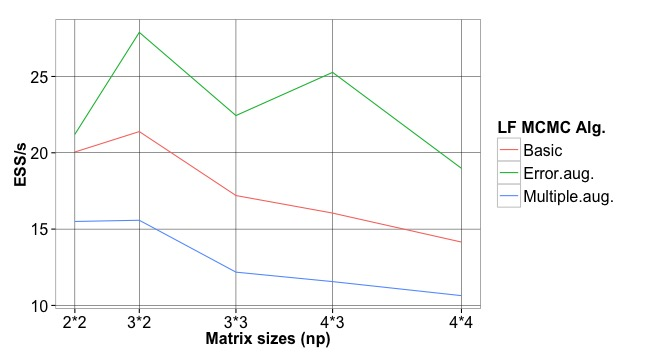
\includegraphics[width=0.60\textwidth]{plot1}
    \caption{Comparing ESS/s for different variants of LF MCMC across various matrix normal sizes}
    \label{fig:ESS/s}
\end{figure}
}

\frame{\frametitle{Conclusion and Future scope}
\begin{itemize}
\item Minkowski distance with $p=3$ and Uniform kernel gave maximum ESS/s for all the variants and matrix sizes.
\vspace{0.1in}
\item Error augmented LF MCMC sampler appears to be performing better in terms of effective sample size per second.
\vspace{0.1in}
\item With increase in matrix sizes, ESS/s decreases for each variant in general. The run times increase exponentially. 
\vspace{0.1in}
\item  It would be interesting to implement the LF methods via Gaussian copula for higher order tensors following normal distribution.
\end{itemize}
}


\bibliography{bibfile}{}
\bibliographystyle{plain} 


\end{document}